		\item Let 
		$\vec{A} = \myvec{1 & 2 & 3 & 4 \\ 4 & 1 & 2 & 3 \\ 3 & 4 & 1 & 2 \\ 2 & 3 & 4 & 1}$
		and 
		$\vec{B} = \myvec{3 & 4 & 1 & 2 \\ 4 & 1 & 2 & 3 \\ 1 & 2 & 3 & 4 \\ 2 & 3 & 4 & 1}$.
		Let $\det\brak{\vec{A}}$ and $\det\brak{\vec{B}}$ denote the determinants of the matrices $\vec{A}$ and $\vec{B}$, respectively.
		Which one of the options given below is TRUE?
\hfill{\brak{\text{CS 2023}}}
		
		\begin{enumerate}
			\begin{multicols}{1}
				\item $\det\brak{\vec{A}} = \det\brak{\vec{B}}$
				\item $\det\brak{\vec{B}} = -\det\brak{\vec{A}}$
				\item $\det\brak{\vec{A}} = 0$
				\item $\det\brak{\vec{A}\vec{B}} = \det\brak{\vec{A}} + \det\brak{\vec{B}}$
			\end{multicols}
		\end{enumerate}
		\item Let $\vec{A}$ be the adjacency matrix of the graph with vertices $\{1, 2, 3, 4, 5\}$.
\begin{figure}[H]
	\centering
	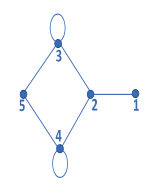
\includegraphics[width=0.3\linewidth]{GATE/2023/CS/figs/screenshot009}
	\caption{}
	\label{fig:screenshot009}
\end{figure}
		Let $\lambda_1, \lambda_2, \lambda_3, \lambda_4$, and $\lambda_5$ be the five eigenvalues of $\vec{A}$. Note that these eigenvalues need not be distinct.
		The value of $\lambda_1 + \lambda_2 + \lambda_3 + \lambda_4 + \lambda_5 = $ \underline{\hspace{2cm}}
		\hfill{\brak{\text{CS 2023}}}
		
